\section{Implementation}

In this section we build on the analysis. In the \nameref{sec:analysis} we described different approaches we could choose to solve different aspects of the generation of the dataset. Now, we will detail on the approaches we chose.


\subsection{Wikidata Preprocessing}
\label{sec:wikidata_preprocessing_implementation}
This module aims to load the wikidata dump file and output three lists. The first list contains QPQ triples, triples of ids representing a relationship (Q173998 P3373 Q187923 for example). The second list provides us with names for the ids mentioned in the first list (Q187923 Ginny Weasley, P3373 sibling). The third one provides the mapping of entity id to the title of the corresponding article if such exists (příklad). Those three lists will serve as the source of structured data.

The first step of our preprocessing is to filter wikidata to remove entities, that we will not use. We require each entity to have at least one Czech name (alias or label), otherwise, there would be no good way to find mentions of that entity later in the entity matching step. CERED creation does not require the Czech names of relations so we will keep all of them.

Apart from the filtering, we should consider whether we might benefit from keeping more information about a relationship (meaning the instantiation of a relation) than just the ids. Wikidata relationships often contain additional information specific for the relation type. For example, some relationships are valid only for some period of time. The minister of magic changes every few years (\todo{typografie} "position held" relationship between Cornelius Fudge and the Ministry of Magic has following additional information attached to it: start time 1990, end time 1996, replaces Millicent Bagnold, replaced by Rufus Scrimgeour). In our use case, as we plan to limit text analysis to the syntactic level, such information is not beneficial. 

The second step addresses removing duplicate relationships that differ only in the additional information tied to the relationship (CBS received many Peabody Awards for example). Such duplicates where the entire QPQ is the same would not be useful in the future and might require special attention in the relation matching step. We will remove even relationships that differ only in the “P” part. If we kept them, in the relation matching we would either create multiple relation mentions (sentence with two tagged entities and the label of their relationship) that only differ in the relationship. CERED is supposed to be a dataset on which it is possible to train a model in a single label classification task. Such mentions would result in the same inputs (sentence with two tagged entities) and different outputs (the relationship label). We could change the format of our dataset to have a set of relations for each mention, but such data is confusing, non-traditional and overall not what we aim for in this thesis. 

After these steps, the first list contains approximately 2 million QPQ triples.

\subsection{Wikitext Parsing}

\label{sec:wikiperia_parsing_implementation}

This module aims to parse wikitext (Wikipedia markup language) from the Czech Wikipedia dump into a clean text with attached information about wikilinks in the original markup.

As we already explained in \nameref{sec:wikipedia_parsing_analysis}, wikitext contains a lot more than fully unstructured data. Different kinds of infoboxes, tables or lists are contained within the sentence-like text. Some of these elements are implemented using the so-called template syntax. Therefore, it would be tempting to simply remove all the text that is contained in a template. The problem is that not all templates are bad. For example, we may use a template to divide the text into two columns containing valid sentences. Therefore, discarding all such data seems unnecessarily harsh.

When developing the methodology for wikitext parsing, there was not a \vuvozovkach{gold} to compare it with. The only means of evaluation we had at the time was repeatedly going through a small set of articles and trying to discard unnecessary data. We tailored the rules for wikitext parsing to these articles in such a way that only sentence-like parts remained. 

Once we implemented the whole CERED generator and were able to see the relation mentions, we realized that the previous method of evaluation was not good enough. Therefore, we adopted a new one, as described in XX (\chybi{nedopsaná sekce v analýza - result evaluation}\todo{do závorky dát jméno metodiky}). We looked at the different histograms and investigated the abnormalities. For example, a lot of sports articles report results of a match (tournament, event?) and these are often stored in custom tables that were not filtered by the rules from the previous paragraph. Moreover, these tables oftentimes contain information about the nationality of the players, resulting in a huge amount of matched entities and relations.

Based on the analysis of all the available data, we decided not to include the following content in the clean text:
\begin{itemize}

\item HTML tags within wikitext
\item headings
\item tables
\item lists
\item templates matching the following patterns: obsazení*, sloupce*, seznam*, příbuzenstvo*, *předkové*, *box*, *locmap*, *tabulka*. (In English: cast*, columns*, lists*, relatives*, *ancestors*, *box*, *locmap*, *table*)
\item wikilinks to categories and files

\end{itemize}
\todo{typografie by mohla být lepší}

One more technical issue we encountered was correctly assigning spans to wikilinks, i.e. where the link starts and ends in the text. We can demonstrate the problem on the following sentence: “The main [[story arc]] concerns Harry's struggle against [[Lord Voldemort]], a dark wizard who intends to become immortal, overthrow the wizard governing body known as the [[Ministry of Magic]] and subjugate all wizards and [[Muggle]]s (non-magical people).” The correct span for Muggles should contain the trailing s even though it is not part of the wikilink itself. In Czech such trailing characters are common. The set of chars that seem to end wikilinks written in such forms are \vuvozovkach{ ,.\textbackslash n}. \todo{vynechat? nevynechat?}

One more thing we mentioned in the analysis about wikitext is the possible boost of performance if the text-part of a wikilink was added to the set of names for the given entity. We exported such names, kept only those that were not already added to wikidata, and read through many of them. This process is time-consuming because one often has to actually look up the entity to know whether a given name is sensible. Even though we do not have any data about the proportion of good and bad names, the overall impression was clearly leaning towards not using such data. The two main reasons were that commonly the name was actually a class name, not instance name (like school linking to Hogwarts). Cases, where the name was just a pronoun, were less frequent but would likely cause much trouble later on.

\subsection{Entity Matching}
\label{sec:entity_matching_implementace}
We discussed in great detail the pros and cons of different entity matching methods, implying that the more complex the matching method, the better. We work with a single language and tools for lexical analysis are available and reliable. Therefore implementing language-independent matching methods (string similarity for example) is not beneficial. 

We load the entity names in a slightly transformed form. We lower the case and add spaces around every dot character We used lexical analyzer to split text to sentences and to obtain features from sentences (tokens, lemmas and lexemes). An entity name (sequence of k strings - tokens - separated by a space) is matched in a sentence if (i) the entity is a candidate entity for the sentence and (ii) there is a sequence of k consecutive tokens in the sentence such that each token in the name is a member of the lexeme of the corresponding token in the sentence. 

We intended to allow a less strict word order, but we were unable to justify such a choice. After reading several articles we did not find any entity mentions that would be newly matched. This might imply that even though word order is relatively free in Czech, noun phrases tend to keep their word order. The other explanation is based more on the fact that a human reader is more likely to recognize entity mention if it is in the standard word order. Looking for entity mention is again more time consuming than it seems, because we do not know, what is a wikidata entity, therefore a lot of looking up is involved and we believe that often we would not have thought that something is a wikidata entity even though it is. Such \vuvozovkach{improvement} could still raise the number of entities matched but probably would lower the precision.

We considered allowing one special case. Most articles are based on one entity, therefore we expect many sentences to mention this entity. Often the entity is mentioned either by a pronoun (pronouns that express the subject are typically omitted in Czech), or by part of its full name.  Přijali ho do školy čar a kouzel v Bradavicích. Když se Harry vydal do Bradavic, našel nového kamaráda Rona Weasleyho. .. Pak už jel \vuvozovkach{domů} a musel přežít další dva měsíce u Dursleyových. We already stated that we will not attempt to deal with pronouns. We tried to propose rules for choosing the correct substring of the entity name. The diversity of wikdata makes such a task extremely difficult. Together with the risk that we would decrease the precision of entity matching we decided to stick with full names only.

In the wikitext parsing section, we prepared spans and ids for wikilinks. We merge these with the ones matched by this module and post-process them. We discard each mention whose span is within a span of different mention of the same entity. This removes duplicates and keeps the one that is more specific.

\chybi{na obrázku s volemortem ukázat, jak to nakonec funguje}

\subsection{Relation Matching}
So far we obtained sentences with tagged entity mentions. For each tuple of entity mentions within the same sentence, we checked if a relationship of those two entities was present in wikidata (using the prepared QPQ list). Given the filtering in wikidata preprocessing we are guaranteed that there is at most one such relationship. 

At this stage, we need to address likely incorrectly matched entities that make the dataset bloat. One example of such bloating that we encountered was in an article about kindergarten\footnote{\url{https://cs.wikipedia.org/w/index.php?oldid=18388144}}, in the sentence \vuvozovkachtextit{Jsou závazná pro předškolní vzdělávání v \textbf{mateřských školách}, v \textbf{mateřských školách} zřízených podle § 16 odst. 9 školského zákona, v lesních \textbf{mateřských školách} a v přípravných třídách základních škol.} thousands of relation mentions were found. Many kindergartens are named Mareřská škola (kindergarten), all of them are an instance of the abstract kindergarten entity and therefore candidate entities. If a sentence contains the term \vuvozovkach{mateřská škola} (or its form), all these entities will be matched. And the relationship “Mateřská škola is a mateřská škola” \todo{typografie} will be assigned many times as well. 

After investigating many other unusual cases, we decided to discard any sentence with at least 10 entity mentions in it. We also tried to experiment with different limits, but the results were unconvincing. For example, increasing the constant to 50 keeps an additional 13\% of relationship mentions but extends the set of sentences only by 1\%.

\chybi{zašuměné histogramy}

\subsection{Characteristics of the Generated Dataset}
The full dataset, which was obtained by the process we described in the previous sections, contains almost one and a half million relation mentions. In the next few paragraphs, we will talk about some more detailed statistic of this dataset - CERED0. 

We found at least one mention in 293591 articles. In these articles, the average number of found mentions is slightly less than 5 and the median is nearly 7. The article with most mentions is Spojené království\footnote{\url{https://cs.wikipedia.org/w/index.php?oldid=18752891}} (United Kingdom). The distribution of mentions in articles is shown \chybi{vložit histogramy}

There are 490501 different sentences that are used in the mentions. We set the limit on entity mentions per sentence to 10. On average there were approximately 3 relation mentions in a sentence (that had at least one mention) and the maximum of 72 mentions per sentence was reached 34 times. The length of sentences ranges from 2 to 401 tokens, the very short ones usually came from templates that were not removed, on the other hand, the very long ones are often caused by incorrectly written articles\footnote{Example of an incorrectly written article \url{https://cs.wikipedia.org/w/index.php?oldid=18723498}}. We tried to remove all templates to see if the range (and distribution) of the number of words improves, but we did not find a significant improvement.



\begin{figure}[h]\centering
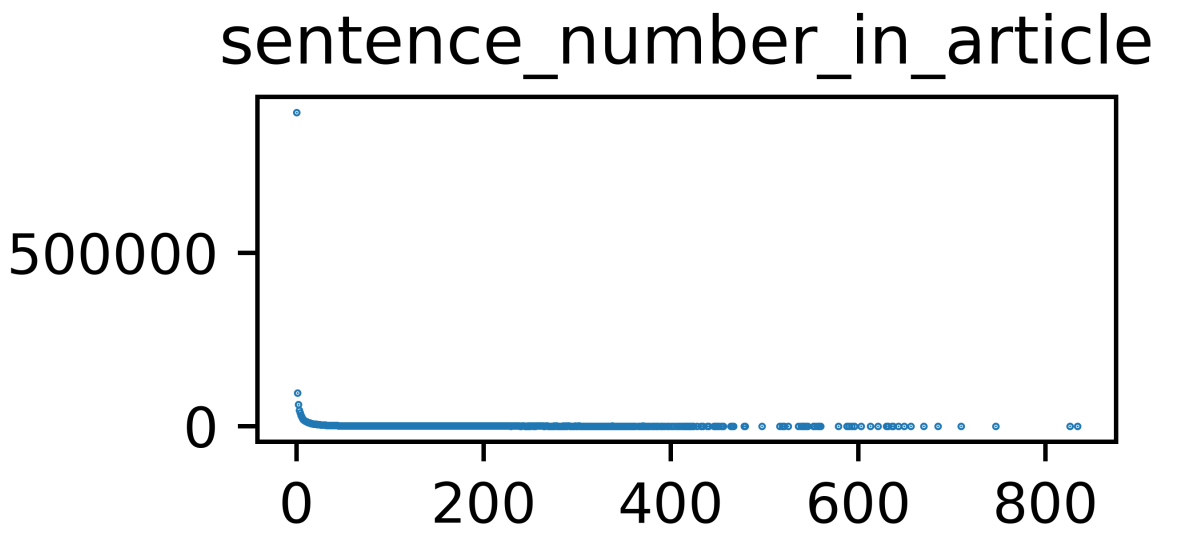
\includegraphics[width=119mm, height=54mm]{./img/CERED0_sentence_number_histogram}
\caption{todo}
\label{obr10:vety_histogram}
\end{figure}


Another possibility is to observe how the position of a sentence in an article influences the number of relation mentions. We expected that the first sentences in an article will contain the highest number of relation mentions. The first sentences tend to contain wikilinks and the use of pronouns or shorter names is limited because each entity has to first be introduced by its full name. As we can see in \autoref{obr10:vety_histogram}, our hypothesis seems to be correct, ant partially applicable to a couple of sentences, not just the first one. 904803 mentions come from sentences that are first in their respective articles. This constitutes over 60\% of all mentions.





\section{CERED Versions}
In this section we describe how and why we decided to postprocess the generated datasets. 

The full CERED is already a valid relationship classification dataset. It has nearly one and a half million mentions, but as we discussed in the previous section, some of them might be of poorer quality than others. In this section, we will describe different versions of CERED with CERED0 being the biggest (least filtered) and CERED4 the smallest. 


Each version is split up into three disjunct sets: train set, dev set and test set. Ideally, the test set would operate on a different set of entities (so that models learn to predict relationships based on sentences, not on the knowledge of entities). We believe that such a restriction is unnecessarily strong. Some entities are mentioned in many articles, which does, in fact, make them part of common knowledge (connected to the language we train on). Instead, we decided to relax the restriction to distinct articles. We sampled two sets of 10000 articles, one for test and one for dev set. In each version of CERED, the same articles are used for dev, test and train.
\subsection{CERED0}
CERED0 is the raw dataset just as we described it in the previous section. We do not artificially change the relation type, so no negative relation is present. We do not recommend this version for direct training, we mostly keep it to preserve the full information obtainable from our generator.

\subsection{CERED1}
CERED1 is close in size to CERED0. We removed long (over 100 words) and short (under 5 words) sentences. We also removed overly represented relations and changed labels of underrepresented relations to \relationtype{other}, which will be the negative relation in CERED1. We will properly define under-represented and over-represented relations in the next paragraph where we describe the CERED2 dataset.

\subsection{CERED2}

CERED1 has 3 potential flaws that we have not addressed, yet. First, one sentence could be included multiple times in a dataset. Second, there were some relations with only a few relation mentions. Third, we did not try to handicap overly represented relatations. 

We try to address these issues in CERED2. We start with CERED1 and for each sentence, if there are multiple relation mentions, we keep only the mention that was the least represented in CERED1, and discard the others. Next, we count the sizes of representations of all mentions and say that a relation is under-represented if it has less than 1000 mentions. We take all the mentions whose relation is considered under-represented and relabel them to \relationtype{other}. This change is also applied to CERED1. After such relabeling, the \relationtype{other} relation still was not the most represented. We decided to discard mentions of the two most represented relations: \relationtype{\wikiitem{instance of}{P31}} and \relationtype{\wikiitem{country}{P17}}.

\begin{table}

\caption{CEREDs statistics.}

\label{table:CEREDsStatistics}

\begin{tabular}{p{2,3cm} r r r r }

\hline
Dataset & \# mentions & Inventory size & Negative \% & Test dataset\\
\hline
\hline
CERED0 & 1 462 546 & 692 & 0 & 25 066\\
CERED1 & 999 287 & 64 & 14.1 & 17 214\\
CERED2 & 374 914 & 64 & 18.8 & 6 530\\
CERED3 & 157 972 & 64 & 22.6 & 2 787\\
CERED4 & 10 766 & 59 & 22.1 & 188\\
\hline


\end{tabular}

\end{table}






\subsection{CERED3}
Even after the restriction on the uniqueness of sentences, half of the CERED2 sentences are the first sentences within the articles they originated from. Such sentences have a rather unique structure that is not as common outside of Wikipedia. This inspired CERED3 which is the remainder of CERED2 after removing all mentions in \vuvozovkach{first} sentences.

\subsection{CERED4}
There are two stages in the CERED generation process that might be relatively unprecise. The entity matching stage and the relation matching stage. CERED4 keeps only the relation mentions from CERED3, in which both entities were manually-labelled directly in wikitext in the form of wikilinks. The CERED4 dataset is, unfortunately, small, but has the highest potential to be precise.


%


\tikzset{lines/.style={draw=none},}


\begin{figure}[h]
\centering
\begin{subfigure}[t]{.5\textwidth}
  \centering
  \hspace{1cm}
\begin{tikzpicture}
  \tikzstyle{every node}=[font=\tiny]
\pie [rotate = 180, hide number,radius =2,style={lines}]{8e+01/No relation,3.6/ ,2.6/ ,2.0/ ,1.3/ ,0.78/ ,0.77/ ,0.71/ ,0.7/ ,0.63/ ,0.54/ ,0.46/ ,0.45/ ,0.43/ ,0.42/ ,0.37/ ,0.33/ ,0.33/ ,0.32/ ,0.3/ ,0.28/ ,0.27/ ,0.26/ ,0.25/ ,0.24/ ,0.22/ ,0.21/ ,0.21/ ,0.16/ ,0.16/ ,0.14/ ,0.14/ ,0.14/ ,0.12/ ,0.11/ ,0.098/ ,0.097/ ,0.097/ ,0.068/ ,0.057/ ,0.05/ ,0.031/ }
\end{tikzpicture}
  \caption{TACRED}
  \label{fig:corridors_input}
\end{subfigure}%
\begin{subfigure}[t]{.5\textwidth}
  \centering
\begin{tikzpicture}
  \tikzstyle{every node}=[font=\tiny]
\pie [rotate = 180, hide number,radius =2,style={lines}]{
1.7e+01/Other, 1.2e+01/ ,1.2e+01/ ,1.1e+01/ ,9.1/ ,8.8/ ,8.6/ ,8.4/ ,6.8/ ,6.2/ }
\end{tikzpicture}
  \caption{S10T8}
  \label{fig:corridors_before}
\end{subfigure}


\begin{subfigure}[t]{.5\textwidth}
  \centering
\begin{tikzpicture}
  \tikzstyle{every node}=[font=\tiny]
\pie [rotate = 180, hide number,radius =2,style={lines}]{1.9e+01/Other,8.4/P150 ,6.7/P131 ,5.9/P279 ,4.6/ ,4.5/ ,3.1/ ,3.0/ ,2.9/ ,2.7/ ,2.7/ ,2.2/ ,2.0/ ,2.0/ ,1.8/ ,1.4/ ,1.4/ ,1.3/ ,1.3/ ,1.2/ ,1.1/ ,0.91/ ,0.89/ ,0.89/ ,0.89/ ,0.85/ ,0.84/ ,0.77/ ,0.67/ ,0.64/ ,0.64/ ,0.63/ ,0.58/ ,0.56/ ,0.55/ ,0.5/ ,0.5/ ,0.48/ ,0.47/ ,0.45/ ,0.44/ ,0.42/ ,0.4/ ,0.4/ ,0.4/ ,0.39/ ,0.39/ ,0.39/ ,0.38/ ,0.37/ ,0.35/ ,0.34/ ,0.34/ ,0.32/ ,0.32/ ,0.32/ ,0.31/ ,0.29/ ,0.29/ ,0.29/ ,0.29/ ,0.29/ ,0.28/ ,0.28/ }
\end{tikzpicture}
  \caption{CERED2}
  \label{fig:corridors_input}
\end{subfigure}%
\begin{subfigure}[t]{.5\textwidth}
  \centering
  \hspace{0.5cm}
\begin{tikzpicture}
  \tikzstyle{every node}=[font=\tiny]
\pie [rotate = 180, hide number,radius =2,style={lines}]{1.9e+01/P17 ,1.3e+01/P31 ,6.7/P131 ,5.9/P106 ,4.8/ ,3.7/ ,3.7/ ,3.4/ ,3.2/ ,2.7/ ,1.5/ ,1.5/ ,1.3/ ,1.3/ ,1.2/ ,1.2/ ,1.1/ ,1.1/ ,0.99/ ,0.97/ ,0.75/ ,0.7/ ,0.66/ ,0.62/ ,0.57/ ,0.52/ ,0.49/ ,0.48/ ,0.44/ ,0.39/ ,0.38/ ,0.37/ ,0.34/ ,0.33/ ,0.32/ ,0.32/ ,0.27/ ,0.27/ ,0.26/ ,0.25/ ,0.25/ ,0.25/ ,0.23/ ,0.23/ ,0.22/ ,0.22/ ,0.21/ ,0.21/ ,0.21/ ,0.19/ ,0.18/ ,0.18/ ,0.18/ ,0.17/ ,0.17/ ,0.17/ ,0.16/ ,0.16/ ,0.15/ ,0.15/ ,0.15/ ,0.15/ ,0.15/ ,0.15/ ,0.14/ ,0.13/ ,0.13/ ,0.13/ ,0.13/ ,0.13/ ,0.12/ ,0.12/ ,0.12/ ,0.11/ ,0.11/ ,0.11/ ,0.11/ ,0.11/ ,0.11/ ,0.11/ ,0.11/ ,0.11/ ,0.1/ ,0.1/ ,0.1/ ,0.1/ ,0.1/ ,0.1/ ,0.098/ ,0.097/ ,0.096/ ,0.093/ ,0.091/ ,0.088/ ,0.088/ ,0.083/ ,0.081/ ,0.081/ ,0.079/ ,0.079/ ,0.076/ ,0.076/ ,0.075/ ,0.073/ ,0.072/ ,0.07/ ,0.07/ ,0.068/ ,0.067/ ,0.066/ ,0.066/ ,0.065/ ,0.065/ ,0.063/ ,0.063/ ,0.061/ ,0.06/ ,0.059/ ,0.058/ ,0.057/ ,0.057/ ,0.057/ ,0.057/ ,0.057/ ,0.054/ ,0.053/ ,0.053/ ,0.053/ ,0.049/ ,0.048/ ,0.048/ ,0.048/ ,0.048/ ,0.047/ ,0.046/ ,0.044/ ,0.043/ ,0.043/ ,0.043/ ,0.041/ ,0.041/ ,0.041/ ,0.039/ ,0.038/ ,0.038/ ,0.036/ ,0.036/ ,0.034/ ,0.032/ ,0.031/ ,0.031/ ,0.031/ ,0.031/ ,0.031/ ,0.031/ ,0.03/ ,0.029/ ,0.029/ ,0.029/ ,0.029/ ,0.029/ ,0.028/ ,0.028/ ,0.028/ ,0.028/ ,0.027/ ,0.027/ ,0.027/ ,0.027/ ,0.027/ ,0.027/ ,0.026/ ,0.025/ ,0.025/ ,0.025/ ,0.025/ ,0.024/ ,0.022/ ,0.022/ ,0.022/ ,0.022/ ,0.021/ ,0.021/ ,0.021/ ,0.021/ ,0.021/ ,0.021/ ,0.021/ ,0.02/ ,0.02/ ,0.019/ ,0.019/ ,0.019/ ,0.019/ ,0.019/ ,0.018/ ,0.018/ ,0.018/ ,0.018/ ,0.018/ ,0.018/ ,0.017/ ,0.017/ ,0.017/ ,0.017/ ,0.016/ ,0.016/ ,0.016/ ,0.015/ ,0.015/ ,0.015/ ,0.014/ ,0.013/ ,0.013/ ,0.013/ ,0.012/ ,0.012/ ,0.012/ ,0.011/ ,0.011/ ,0.011/ ,0.011/ ,0.011/ ,0.01/ ,0.01/ ,0.01/ ,0.01/ ,0.01/ }

\end{tikzpicture}
  \caption{CERED0}
\end{subfigure}
\caption{Representation of relations in different relationship extraction datasets. In CERED0, only top 250 relations are shown, the rest corresponds to the empty sector above P17. We only kept the most relevant labels.}
\label{fig:kolace}
\end{figure}





\subsection{Other Considered Variations}
\label{sec:otherconsideredvariations}
When curating the CEREDs we considered many different criteria. For example, we chose the constant 1000 for underrepresented relations after several experiments. The good thing about this value is that only two relations were more dominant than the new \relationtype{other} relation and at the same time, we would keep 63 positive relations. We wanted our dataset to be at least somewhat comparable to other datasets in the proportion of data and inventory size. S10T8 contains 10717 mentions and 10 relations, TACRED contains around 100 000 mentions and 41 relations. The size of Riedel NYT depends, just like its inventory, on what data is used (and whether duplicates are removed and so on). We worked with nearly 700 000 mentions and 58 relations. Since the sizes of CERED1-3 range from approximately a million to approximately 160 000 mentions, we wanted the size to be around 50 or 60. The distributions of relations in different datasets is captured in \autoref{obr:relations}.



\begin{figure}[h]\centering
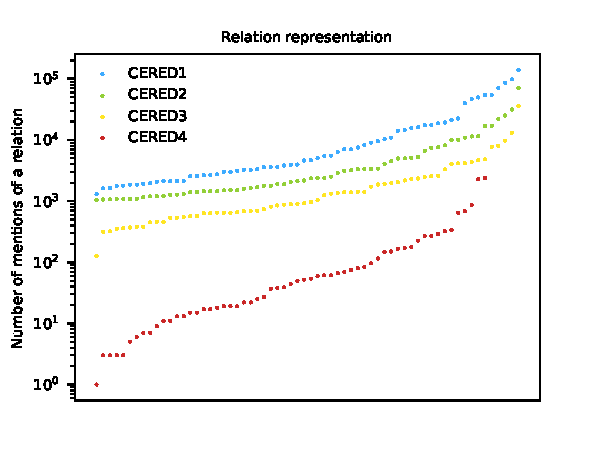
\includegraphics[scale=1]{./img/Relations1-4}
\caption{Sizes of relation representations. For each we ordered the relations by their frequency.}
\label{obr:relations}
\end{figure}

\paragraph{Named entities.}

One more labour intensive variation we wanted to create was supposed to be focused on named entities. We tried to curate a set of named entity types (such as person, place, etc.) based on wikidata, in order to later use them as additional information during training. 

We used the QPQ triples described in the \nameref{sec:wikidata_preprocessing_implementation} section to create an oriented graph with two types of edges. The first edge type - instance edges - connect wikidata items Q\textsubscript{1} and Q\textsubscript{2} if there is a triple Q\textsubscript{1}P31Q\textsubscript{2}, where P31 is the wikidata property \wikiitem{instance of}{P31}, the second type - subclass edges - are added for the \wikiitem{subclass of}{P279} property. The goal of the graph is to capture the transitive nature of the two properties, i.e. if Harry Potter is an instance of a fictional human and fictional human is a subclass of a human, we can assume that Harry Potter is a human. We consider a wikidata item to be a named entity if it is an instance of some other item. If we are interested in all the named entities belonging to some entity type (node in the graph), we can simply find all the named entities for which there is a path between the type and the entity.

We hoped that with such representation, we will be able to curate reasonable set of types. For example, we might want to have a \vuvozovkach{human} entity type and we might intuitively expect \wikiitem{Harry Potter}{Q3244512} (fictional human) to be human. However, as he is fictional, he is not considered to be human in the wikidata ontology. Such an issue can be easily solved by having a \vuvozovkach{person} entity type instead of \vuvozovkach{human}. The problem is that there are just too many similar problems and it is out of scope for this thesis to properly analyze the whole wikidata ontology. 


